\documentclass[12pt]{article}
\usepackage{amsmath}
\usepackage{gvv-book}
\usepackage{gvv}

\title{\textbf{4.13.10}}
\author{\textbf{Aditya Mishra - EE25BTECH}}
\date{September 30, 2025}

\begin{document}

\maketitle

\section*{Question}

The vertices of a triangle are 
\[
\vec{A} = \myvec{-1 \\ -7}, \quad 
\vec{B} = \myvec{5 \\ 1}, \quad 
\vec{C} = \myvec{1 \\ 10}.
\]
Find the equation of the bisector of the angle \(\angle ABC\).

\section*{Solution}

Define vectors  
\begin{equation}
\vec{D} = \vec{A} - \vec{B} = \myvec{-1 - 5 \\-7 - 1} = \myvec{-6 \\ -8},
\end{equation}
\begin{equation}
\vec{E} = \vec{C} - \vec{B} = \myvec{1 - 5 \\ 10 - 1} = \myvec{-4 \\ 9}.
\end{equation}

Compute magnitudes:
\begin{equation}
\|\vec{D}\| = \sqrt{(-6)^2 + (-8)^2} = 10,
\end{equation}
\begin{equation}
\|\vec{E}\| = \sqrt{(-4)^2 + 9^2} = \sqrt{97}.
\end{equation}

Normalize:
\begin{equation}
\vec{e}_{D} = \frac{1}{10} \myvec{-6 \\ -8},
\end{equation}
\begin{equation}
\vec{e}_{E} = \frac{1}{\sqrt{97}} \myvec{-4 \\ 9}.
\end{equation}

The angle bisector vector \(\vec{L}\) is along the sum of normalized vectors:
\begin{equation}
\vec{L} = \vec{e}_{D} + \vec{e}_{E} 
= \myvec{-\frac{6}{10} - \frac{4}{\sqrt{97}} \\[6pt]
       -\frac{8}{10} + \frac{9}{\sqrt{97}}}.
\end{equation}

The line along the bisector passes through \(\vec{B}\), so the vector equation is:
\begin{equation}
\vec{x} = \vec{B} + \lambda \vec{L}, \quad \lambda \in \mathbb{R}.
\end{equation}

\begin{equation}
\Rightarrow \vec{x} = \myvec{5 \\ 1} + \lambda \myvec{-\frac{6}{10} - \frac{4}{\sqrt{97}} \\[6pt]
       -\frac{8}{10} + \frac{9}{\sqrt{97}} }.
\end{equation}

This is the equation of the bisector of \(\angle ABC\).

\section*{Plot}
\begin{figure}[H]
    \centering
    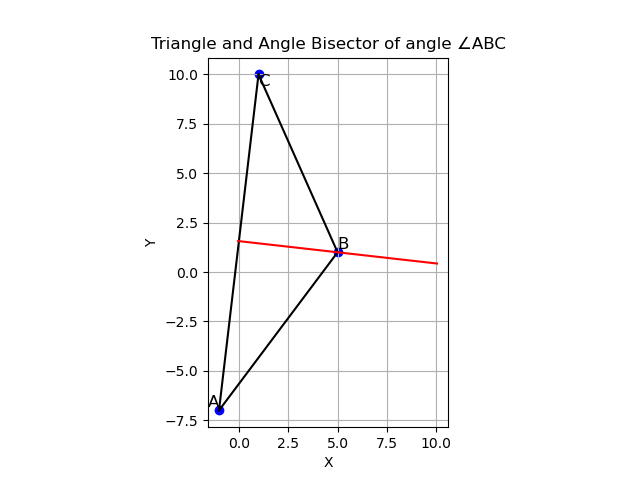
\includegraphics[width=1\columnwidth]{Figs/Figure_1.png}
\end{figure}
\end{document}

